\lecture{12}{02 May 2023}{Review before Midterm 2}

\subsection{Change of Basis}

Consider the \textbf{identity map}, that is
\[
    \begin{array}{ccc}
        V                               & \xlongrightarrow{id} & V                                   \\
        \calb = \{v_1, v_2, \dots, v_n\} &                      & \calb '= \{v'_1, v'_2, \dots, v'_n\} \\
        v_i                             & \mapsto              & v_i
    \end{array}
\]

Note that this is not the map \textbf{represented} by the identity matrix, which would essentially just map the coordinates to be the same between 2 bases.

The matrix \(C = [id]_{\calb, \calb '}\) is the \textbf{change of basis matrix}. Essentially all vectors are kept the same (it's an identity mapping!), but just the coordinates are changed (because the basis changed!).

In particular, this mapping would map:
\begin{align*}
    v_i             & \mapsto C_{i1}v'_1 + C_{i2} v'_2 + \cdots C_{in} v'_n \\
    \begin{pmatrix}
        0      \\
        \vdots \\
        1      \\
        \vdots \\
        0
    \end{pmatrix} & \mapsto C \begin{pmatrix}
                                  0      \\
                                  \vdots \\
                                  1      \\
                                  \vdots \\
                                  0
                              \end{pmatrix} = \begin{pmatrix}
                                                  C_{i1} \\
                                                  \vdots \\
                                                  C_{ij} \\
                                                  \vdots \\
                                                  C_{in}
                                              \end{pmatrix}
\end{align*}

Consider the following: 



\tikzset{every picture/.style={line width=0.75pt}} %set default line width to 0.75pt        

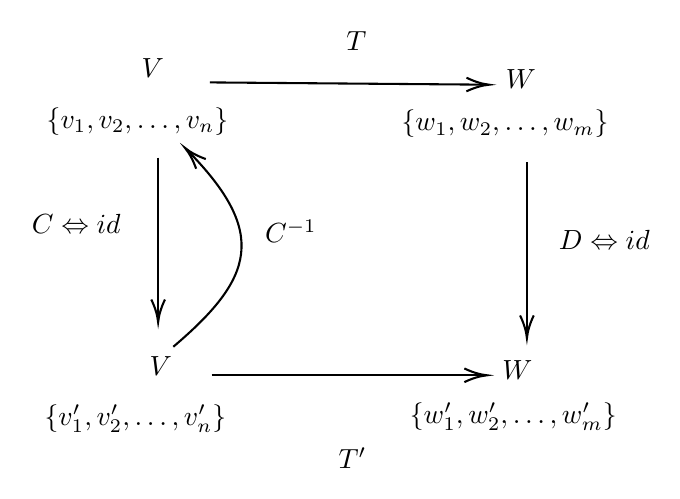
\begin{tikzpicture}[x=0.75pt,y=0.75pt,yscale=-1,xscale=1]
    %uncomment if require: \path (0,282); %set diagram left start at 0, and has height of 282

    %Straight Lines [id:da361443360661001] 
    \draw    (223.19,89.84) -- (223.19,167.09) ;
    \draw [shift={(223.19,169.09)}, rotate = 270] [color={rgb, 255:red, 0; green, 0; blue, 0 }  ][line width=0.75]    (10.93,-3.29) .. controls (6.95,-1.4) and (3.31,-0.3) .. (0,0) .. controls (3.31,0.3) and (6.95,1.4) .. (10.93,3.29)   ;
    %Straight Lines [id:da6566058534654999] 
    \draw    (248.94,194.67) -- (379.67,194.67) ;
    \draw [shift={(381.67,194.67)}, rotate = 180] [color={rgb, 255:red, 0; green, 0; blue, 0 }  ][line width=0.75]    (10.93,-3.29) .. controls (6.95,-1.4) and (3.31,-0.3) .. (0,0) .. controls (3.31,0.3) and (6.95,1.4) .. (10.93,3.29)   ;
    %Straight Lines [id:da28142329892579054] 
    \draw    (400.87,91.99) -- (400.87,174.78) ;
    \draw [shift={(400.87,176.78)}, rotate = 270] [color={rgb, 255:red, 0; green, 0; blue, 0 }  ][line width=0.75]    (10.93,-3.29) .. controls (6.95,-1.4) and (3.31,-0.3) .. (0,0) .. controls (3.31,0.3) and (6.95,1.4) .. (10.93,3.29)   ;
    %Straight Lines [id:da736678524194871] 
    \draw    (248.13,53.56) -- (380.67,54.65) ;
    \draw [shift={(382.67,54.67)}, rotate = 180.47] [color={rgb, 255:red, 0; green, 0; blue, 0 }  ][line width=0.75]    (10.93,-3.29) .. controls (6.95,-1.4) and (3.31,-0.3) .. (0,0) .. controls (3.31,0.3) and (6.95,1.4) .. (10.93,3.29)   ;
    %Curve Lines [id:da7320490255847802] 
    \draw    (230.51,180.92) .. controls (269.28,148) and (276.52,126.11) .. (237.3,86.29) ;
    \draw [shift={(236.1,85.08)}, rotate = 45.01] [color={rgb, 255:red, 0; green, 0; blue, 0 }  ][line width=0.75]    (10.93,-3.29) .. controls (6.95,-1.4) and (3.31,-0.3) .. (0,0) .. controls (3.31,0.3) and (6.95,1.4) .. (10.93,3.29)   ;

    % Text Node
    \draw (213.78,40.66) node [anchor=north west][inner sep=0.75pt]    {$V$};
    % Text Node
    \draw (217.59,184.22) node [anchor=north west][inner sep=0.75pt]    {$V$};
    % Text Node
    \draw (387.51,186.32) node [anchor=north west][inner sep=0.75pt]    {$W$};
    % Text Node
    \draw (389.26,45.89) node [anchor=north west][inner sep=0.75pt]    {$W$};
    % Text Node
    \draw (160.84,115.56) node [anchor=north west][inner sep=0.75pt]    {$C \Leftrightarrow id$};
    % Text Node
    \draw (414.83,123.1) node [anchor=north west][inner sep=0.75pt]    {$D \Leftrightarrow id$};
    % Text Node
    \draw (308.63,228.11) node [anchor=north west][inner sep=0.75pt]    {$T'$};
    % Text Node
    \draw (312.44,27.69) node [anchor=north west][inner sep=0.75pt]    {$T$};
    % Text Node
    \draw (273.19,118.56) node [anchor=north west][inner sep=0.75pt]    {$C^{-1}$};
    % Text Node
    \draw (168,64.4) node [anchor=north west][inner sep=0.75pt]    {$\{v_{1} ,v_{2} , \dots ,v_{n}\}$};
    % Text Node
    \draw (339,65.4) node [anchor=north west][inner sep=0.75pt]    {$\{w_{1} , w_{2} , \dots ,w_{m}\}$};
    % Text Node
    \draw (167,207.4) node [anchor=north west][inner sep=0.75pt]    {$\{v'_{1} ,v'_{2} , \dots ,v'_{n}\}$};
    % Text Node
    \draw (343,206.4) node [anchor=north west][inner sep=0.75pt]    {$\{w'_{1} ,w'_{2} ,\dots ,w'_{m}\}$};
\end{tikzpicture}


then \[
T' = DTC^{-1}
\]
simply tracing back!

In a specific case,


\tikzset{every picture/.style={line width=0.75pt}} %set default line width to 0.75pt        

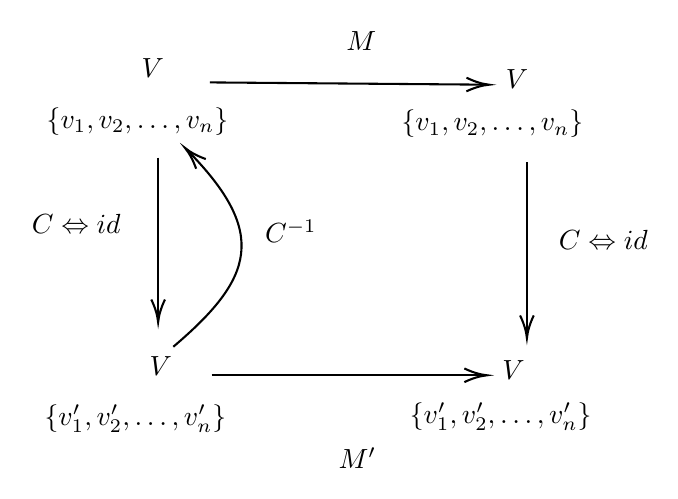
\begin{tikzpicture}[x=0.75pt,y=0.75pt,yscale=-1,xscale=1]
    %uncomment if require: \path (0,282); %set diagram left start at 0, and has height of 282

    %Straight Lines [id:da361443360661001] 
    \draw    (223.19,89.84) -- (223.19,167.09) ;
    \draw [shift={(223.19,169.09)}, rotate = 270] [color={rgb, 255:red, 0; green, 0; blue, 0 }  ][line width=0.75]    (10.93,-3.29) .. controls (6.95,-1.4) and (3.31,-0.3) .. (0,0) .. controls (3.31,0.3) and (6.95,1.4) .. (10.93,3.29)   ;
    %Straight Lines [id:da6566058534654999] 
    \draw    (248.94,194.67) -- (379.67,194.67) ;
    \draw [shift={(381.67,194.67)}, rotate = 180] [color={rgb, 255:red, 0; green, 0; blue, 0 }  ][line width=0.75]    (10.93,-3.29) .. controls (6.95,-1.4) and (3.31,-0.3) .. (0,0) .. controls (3.31,0.3) and (6.95,1.4) .. (10.93,3.29)   ;
    %Straight Lines [id:da28142329892579054] 
    \draw    (400.87,91.99) -- (400.87,174.78) ;
    \draw [shift={(400.87,176.78)}, rotate = 270] [color={rgb, 255:red, 0; green, 0; blue, 0 }  ][line width=0.75]    (10.93,-3.29) .. controls (6.95,-1.4) and (3.31,-0.3) .. (0,0) .. controls (3.31,0.3) and (6.95,1.4) .. (10.93,3.29)   ;
    %Straight Lines [id:da736678524194871] 
    \draw    (248.13,53.56) -- (380.67,54.65) ;
    \draw [shift={(382.67,54.67)}, rotate = 180.47] [color={rgb, 255:red, 0; green, 0; blue, 0 }  ][line width=0.75]    (10.93,-3.29) .. controls (6.95,-1.4) and (3.31,-0.3) .. (0,0) .. controls (3.31,0.3) and (6.95,1.4) .. (10.93,3.29)   ;
    %Curve Lines [id:da7320490255847802] 
    \draw    (230.51,180.92) .. controls (269.28,148) and (276.52,126.11) .. (237.3,86.29) ;
    \draw [shift={(236.1,85.08)}, rotate = 45.01] [color={rgb, 255:red, 0; green, 0; blue, 0 }  ][line width=0.75]    (10.93,-3.29) .. controls (6.95,-1.4) and (3.31,-0.3) .. (0,0) .. controls (3.31,0.3) and (6.95,1.4) .. (10.93,3.29)   ;

    % Text Node
    \draw (213.78,40.66) node [anchor=north west][inner sep=0.75pt]    {$V$};
    % Text Node
    \draw (217.59,184.22) node [anchor=north west][inner sep=0.75pt]    {$V$};
    % Text Node
    \draw (387.51,186.32) node [anchor=north west][inner sep=0.75pt]    {$V$};
    % Text Node
    \draw (389.26,45.89) node [anchor=north west][inner sep=0.75pt]    {$V$};
    % Text Node
    \draw (160.84,115.56) node [anchor=north west][inner sep=0.75pt]    {$C \Leftrightarrow id$};
    % Text Node
    \draw (414.83,123.1) node [anchor=north west][inner sep=0.75pt]    {$C \Leftrightarrow id$};
    % Text Node
    \draw (308.63,228.11) node [anchor=north west][inner sep=0.75pt]    {$M'$};
    % Text Node
    \draw (312.44,27.69) node [anchor=north west][inner sep=0.75pt]    {$M$};
    % Text Node
    \draw (273.19,118.56) node [anchor=north west][inner sep=0.75pt]    {$C^{-1}$};
    % Text Node
    \draw (168,64.4) node [anchor=north west][inner sep=0.75pt]    {$\{v_{1} ,v_{2} , \dots ,v_{n}\}$};
    % Text Node
    \draw (339,65.4) node [anchor=north west][inner sep=0.75pt]    {$\{v_{1} ,v_{2} , \dots ,v_{n}\}$};
    % Text Node
    \draw (167,207.4) node [anchor=north west][inner sep=0.75pt]    {$\{v'_{1} ,v'_{2} , \dots ,v'_{n}\}$};
    % Text Node
    \draw (343,206.4) node [anchor=north west][inner sep=0.75pt]    {$\{v'_{1} ,v'_{2} , \dots ,v'_{n}\}$};
\end{tikzpicture}


then \[
M' = CMC^{-1}
\]

\subsection{Eigenspaces}
If \(\alpha\) is an eigenvalue of \(T\), \(V_\alpha  \coloneqq \{v \mid Tv = \alpha v\} = \ker (T - \alpha I_n)\).

\begin{exercise}
If \(\alpha \neq \beta, V_\alpha \cap V_\beta = \{0\}\)
\end{exercise}